\documentclass[aspectratio=169]{beamer}
% ============================================================
% Beamer presentation — Bitcoin Price Prediction
% Generic version (no per-presenter coordination)
% ============================================================

% ---------------- Theme ----------------
\usetheme{Madrid}
\usecolortheme{seahorse}
\useoutertheme{infolines}
\useinnertheme{circles}
\setbeamertemplate{navigation symbols}{}
\setbeamertemplate{blocks}[rounded][shadow=false]
\setbeamertemplate{title page}[default][colsep=-4bp,rounded=false]
\setbeamerfont{frametitle}{size=\large,series=\bfseries}
\setbeamerfont{title}{size=\LARGE,series=\bfseries}

\definecolor{accentblue}{RGB}{25,72,135}
\definecolor{accentgreen}{RGB}{46,120,72}
\definecolor{accentorange}{RGB}{205,120,40}
\definecolor{accentred}{RGB}{170,40,60}
\setbeamercolor{structure}{fg=accentblue}
\setbeamercolor{frametitle}{fg=white,bg=accentblue}
\setbeamercolor{title}{fg=accentblue}
\setbeamercolor{block title}{fg=white,bg=accentblue}

% ---------------- Packages ----------------
\usepackage{graphicx}
\graphicspath{{Deep_learning_project_2026/}}
\usepackage{booktabs}
\usepackage{amsmath,amssymb}
\usepackage{xcolor}
\usepackage{colortbl}
\usepackage{tikz}
\usetikzlibrary{positioning}
\usepackage{multirow}
\usepackage{array}
\newcolumntype{L}[1]{>{\raggedright\arraybackslash}p{#1}}
\pdfstringdefDisableCommands{\def\translate#1{#1}}
\hfuzz=6pt
\vfuzz=5pt

% ---------------- Title ----------------
\title[Honest Bitcoin Forecasting]{Predicting Bitcoin Honestly}
\subtitle{Log-Return Targets, Walk-Forward Validation, \\
  and Why Sub-1\% MAPE Isn't What It Seems}
\author[Alsuwaidi, Amer, Aljaroodi]{%
  Shamsa Alsuwaidi \and
  Saeeda Amer \and
  Amna Aljaroodi}
\institute[MAI 604]{School of Engineering, Applied Sciences, and Technology \\
  MAI 604 --- Deep Learning \\
  Instructor: Dr.\ Firuz Kamalov}
\date{April 2026}

% ============================================================
\begin{document}
% ============================================================

% =========== TITLE ==========================================
\begin{frame}
  \titlepage
\end{frame}

% =========== CONTRIBUTIONS ==================================
\begin{frame}{Team Contributions}
\footnotesize
\renewcommand{\arraystretch}{1.25}
\begin{columns}[T,onlytextwidth]

\column{0.33\textwidth}
\setbeamercolor{block title}{fg=white,bg=accentblue}
\begin{block}{\color{white}Shamsa Alsuwaidi}
\textbf{Data \& Preprocessing}
\begin{itemize}\scriptsize
  \item Data acquisition (BTC-USD, cross-assets, macro, sentiment)
  \item EDA, missing-value handling, forward-filling
  \item Feature engineering (17 stationary features)
  \item Halving-cycle sin/cos encoding
  \item Leak-free StandardScaler pipeline
  \item Multi-step sequence + anchor construction
  \item Train/Val/Test chronological split
\end{itemize}
\end{block}

\column{0.33\textwidth}
\setbeamercolor{block title}{fg=white,bg=accentgreen}
\begin{block}{\color{white}Saeeda Amer}
\textbf{Models \& Training}
\begin{itemize}\scriptsize
  \item DNN with feature-attention gate
  \item LSTM with temporal self-attention
  \item CNN-Transformer hybrid
  \item Temporal Convolutional Network (TCN)
  \item Unified training protocol (AdamW + Huber + cosine)
  \item Early stopping + gradient clipping
  \item Ensemble combination (avg + val-weighted)
\end{itemize}
\end{block}

\column{0.33\textwidth}
\setbeamercolor{block title}{fg=white,bg=accentorange}
\begin{block}{\color{white}Amna Aljaroodi}
\textbf{Evaluation \& Analysis}
\begin{itemize}\scriptsize
  \item Six-metric evaluation suite (RMSE/MAE/MAPE/$R^2$/DA/F1)
  \item Naive random-walk baseline
  \item 20-fold walk-forward validation
  \item Diebold--Mariano significance testing
  \item Feature-group ablation study
  \item MC Dropout uncertainty quantification
  \item Real-time inference + final report
\end{itemize}
\end{block}

\end{columns}

\vspace{0.4cm}
\centering
\footnotesize\textit{All members contributed to writing the report and preparing this presentation.}
\end{frame}

% =========== OUTLINE ========================================
\begin{frame}{Outline}
\tableofcontents
\end{frame}

% ============================================================
%  PART 1 --- BACKGROUND
% ============================================================

\section{Background \& Motivation}

\begin{frame}{Why predict Bitcoin? And why is it hard?}
\begin{columns}[T,onlytextwidth]
\column{0.53\textwidth}
\textbf{Bitcoin today}
\begin{itemize}
  \item Market cap $>$ \$1.8 trillion
  \item Traded 24/7 across dozens of exchanges
  \item Accessible via spot ETFs (SEC-approved Jan 2024)
  \item Historical high above \$94{,}000
\end{itemize}

\vspace{0.3cm}
\textbf{Why it's hard}
\begin{itemize}
  \item Non-stationary price levels (\$1k $\to$ \$100k+)
  \item Heavy-tailed return distribution
  \item Regime changes (bull runs, crashes, halvings)
  \item Exogenous shocks (regulation, macro news)
\end{itemize}

\column{0.45\textwidth}
\begin{center}
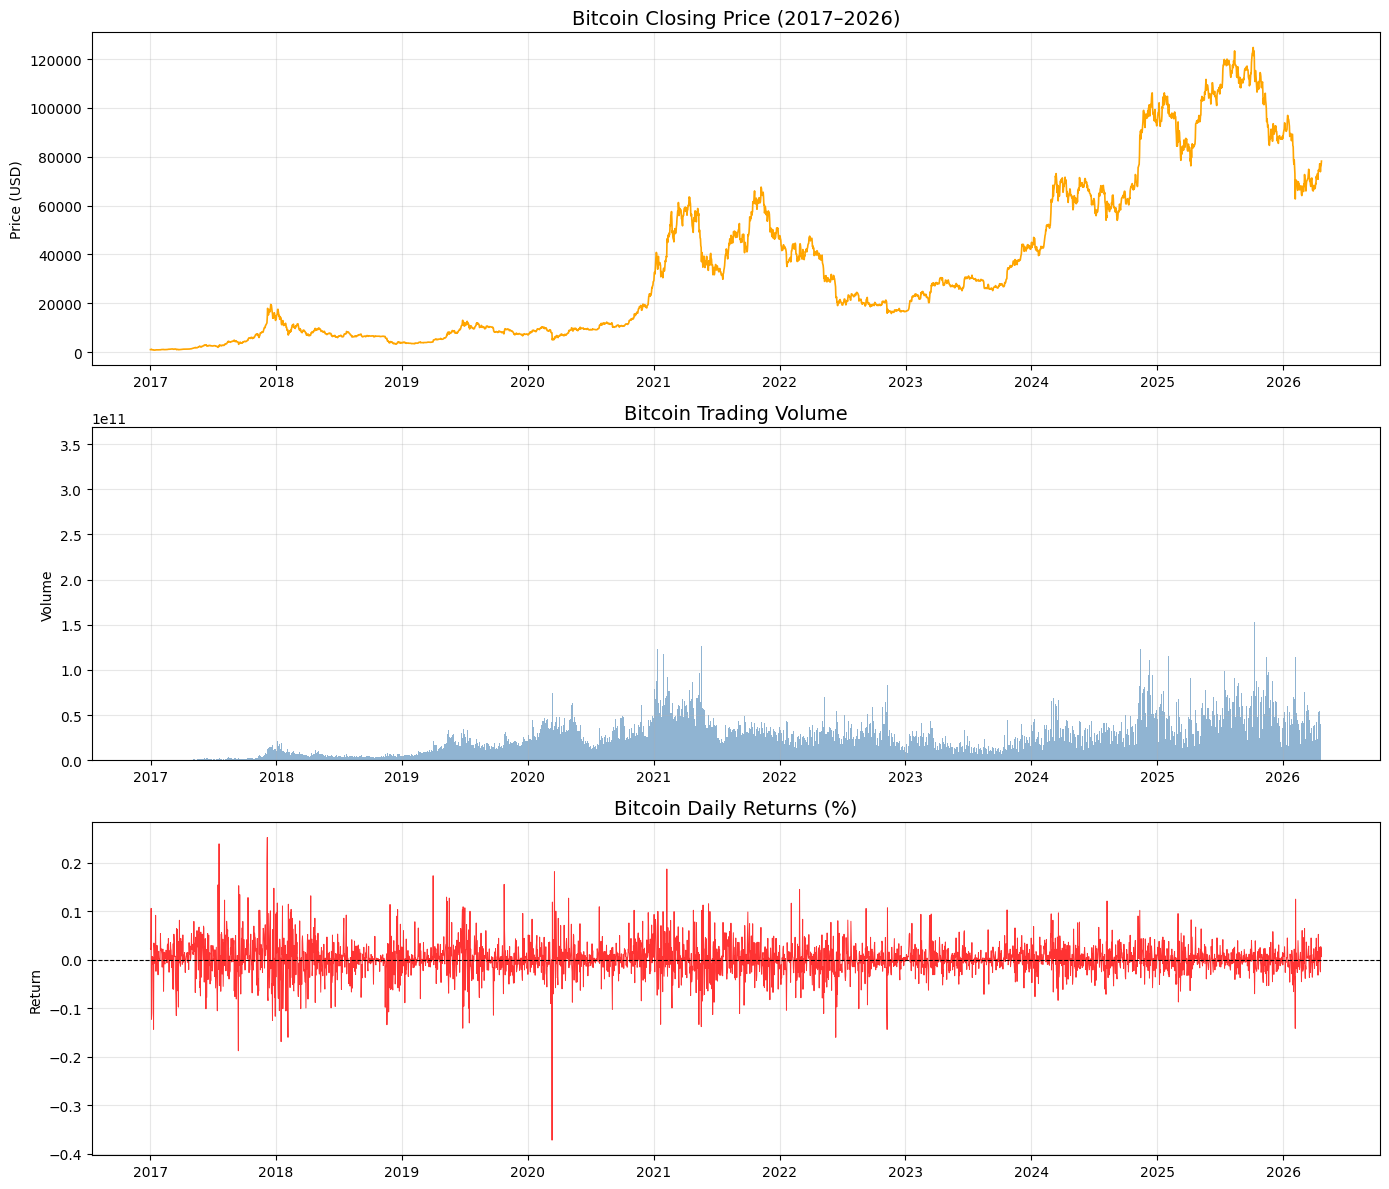
\includegraphics[width=\linewidth]{fig01_eda_bitcoin.png}\\
\scriptsize Closing price, volume, daily returns 2017--2026
\end{center}
\end{columns}
\end{frame}

\begin{frame}{The research question}
\begin{block}{Central question}
Which deep learning architecture --- DNN, LSTM with attention, CNN-Transformer, or TCN --- produces the most accurate next-day Bitcoin forecasts \textbf{under a rigorous, leak-free evaluation protocol}?
\end{block}

\vspace{0.3cm}
\begin{block}{Secondary questions}
\begin{itemize}
  \item Does an ensemble beat the best individual model?
  \item Which \emph{feature groups} (technical / sentiment / cross-asset / macro) actually matter?
  \item Are reported differences between models \emph{statistically significant} or just noise?
\end{itemize}
\end{block}
\end{frame}

\begin{frame}{What the literature says}
\footnotesize
\begin{table}
\renewcommand{\arraystretch}{1.1}
\begin{tabular}{lll}
\toprule
\textbf{Year} & \textbf{Approach} & \textbf{Reported MAPE} \\
\midrule
Hamayel \& Owda (2021) & GRU on daily BTC                    & 0.245\% \\
Jin \& Li (2023)       & VMD-AGRU-RESVMD-LSTM                & 0.394\% \\
Kim et al.\ (2022)     & SAM-LSTM + on-chain                 & 1.33\% \\
Zhang, Li \& Yan (2022)& SDAE-B                              & 1.60\% \\
Chen (2023)            & Random Forest                       & 3.29\% \\
Ji, Kim \& Im (2019)   & DNN                                 & 3.61\% \\
Ye et al.\ (2022)      & LSTM+GRU stacking + Twitter         & 4.49\% \\
\rowcolor{accentblue!15}
\textbf{Wu et al.\ (2025)} & \textbf{Combinatorial Fusion Analysis} & \textbf{0.19\%} \\
\rowcolor{accentgreen!15}
\textbf{Jin et al.\ (2025)} & \textbf{TCN on 1-minute data}     & \textbf{0.002\%} \\
\bottomrule
\end{tabular}
\end{table}

\vspace{0.2cm}
\begin{alertblock}{Red flag}
Reported MAPE spans \textbf{two orders of magnitude} on similar data. Something is off with the evaluation protocols.
\end{alertblock}
\end{frame}

\begin{frame}{The two reference papers we built on}
\begin{columns}[T,onlytextwidth]
\column{0.5\textwidth}
\setbeamercolor{block title}{fg=white,bg=accentblue}
\begin{block}{Wu et al.\ (2025) --- CFA}
Combine 5 base models via:
\begin{itemize}\footnotesize
  \item Score / rank fusion
  \item 104 combination strategies
  \item Diversity-weighted selection
\end{itemize}
Reported MAPE: \textbf{0.19\%}
\vspace{0.2cm}
\\ \textcolor{accentred}{\textbf{Issue:}} Per-day oracle selection across 104 combinations \emph{after} seeing ground truth.
\end{block}

\column{0.5\textwidth}
\setbeamercolor{block title}{fg=white,bg=accentgreen}
\begin{block}{Jin et al.\ (2025) --- TCN}
Dilated causal convolutions on:
\begin{itemize}\small
  \item 1-minute BTC data
  \item Multi-factor features
  \item OHLC + volume + trades
\end{itemize}
Reported MAPE: \textbf{0.002\%}
\vspace{0.2cm}
\\ \textcolor{accentred}{\textbf{Issue:}} 1-min MAPE is not comparable to daily MAPE.
\end{block}
\end{columns}

\vspace{0.3cm}
\centering
\small We take the \textbf{good ideas} (fusion, TCN architecture) but fix the evaluation.
\end{frame}

\begin{frame}{The silent bug in daily BTC forecasting}
\begin{columns}[T,onlytextwidth]
\column{0.5\textwidth}
\textbf{Failure mode \#1 --- Scaler leakage}
\begin{itemize}
  \item Fit \texttt{MinMaxScaler} on \emph{all} data
  \item Train set lives in $[0, 0.3]$
  \item Test set lives in $[0.7, 1.0]$
  \item Model \emph{cannot} reach test-range values
\end{itemize}

\vspace{0.4cm}
\textbf{Failure mode \#2 --- Non-stationary target}
\begin{itemize}
  \item Predict \emph{price level} directly
  \item Price trends from \$1k to \$100k+
  \item Neural nets do not extrapolate
  \item Model outputs stuck in training range
\end{itemize}

\column{0.5\textwidth}
\begin{alertblock}{What we saw before the fix}
\centering
\begin{tabular}{ll}
$R^2$ of CNN-Transformer & $-16.64$ \\
$R^2$ of DNN & $-5.56$ \\
$R^2$ of LSTM & $-2.16$ \\
MAPE & $\approx 50\%$
\end{tabular}
\end{alertblock}

\vspace{0.3cm}
\begin{block}{The fix, in one line}
Predict \textbf{log returns} on features scaled using \textbf{training rows only}.
\end{block}
\end{columns}
\end{frame}

% ============================================================
%  PART 2 --- SYSTEM PIPELINE
% ============================================================

\section{System Pipeline}

\begin{frame}{End-to-end pipeline}
\centering
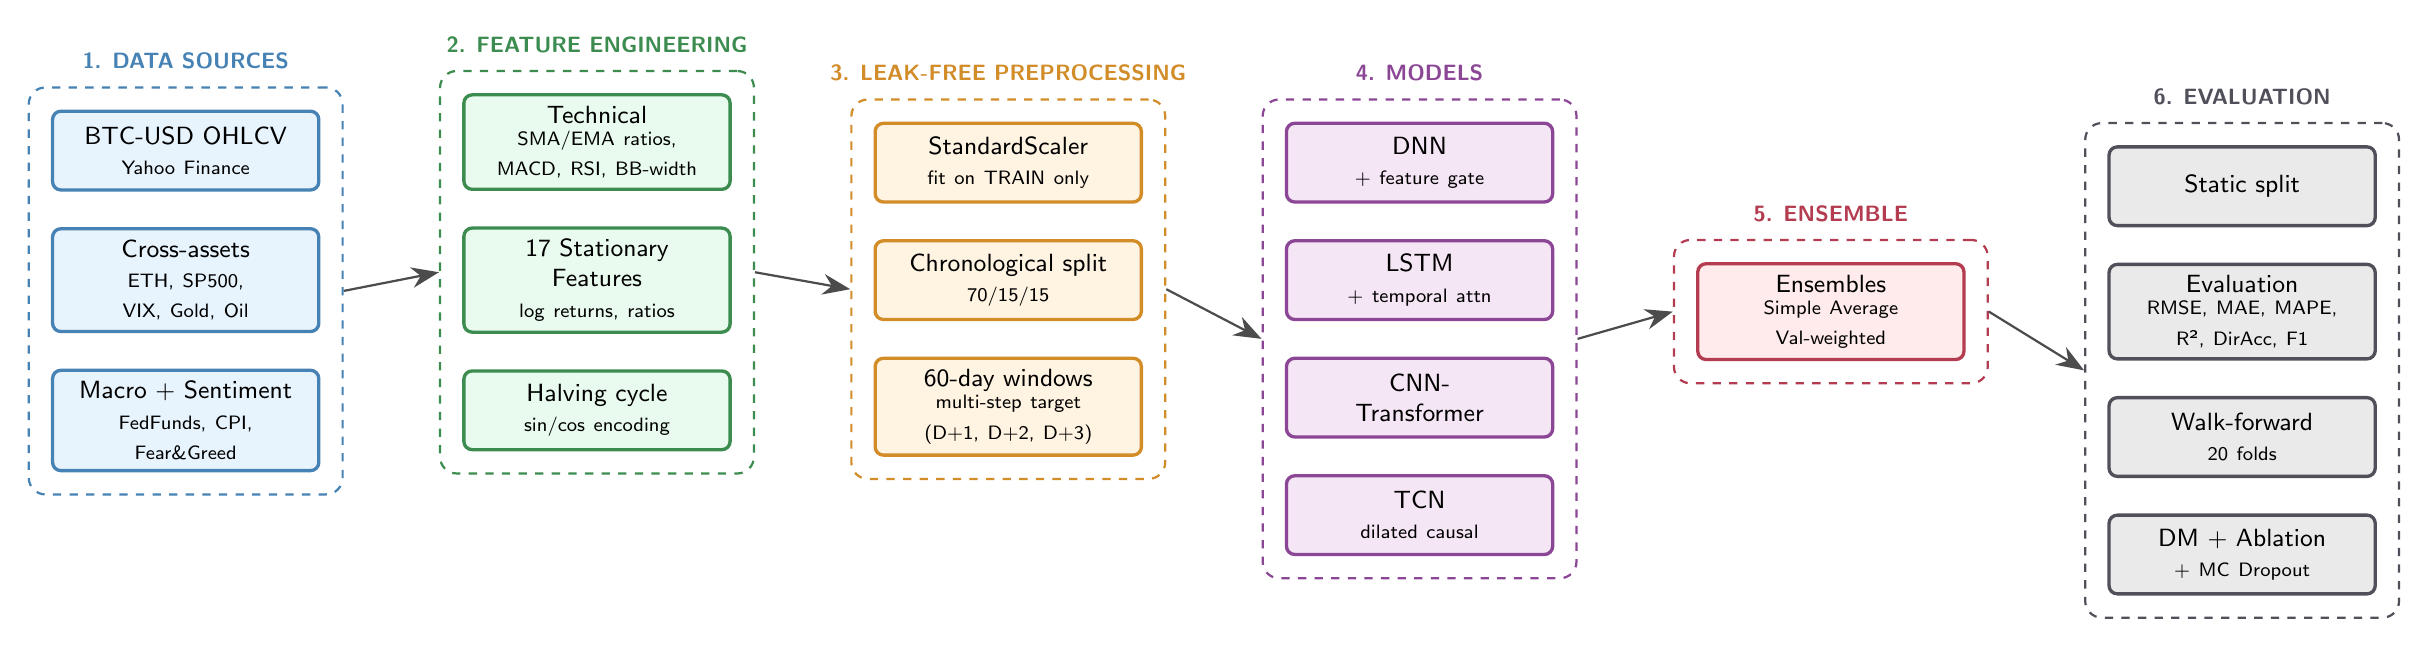
\includegraphics[width=0.98\textwidth]{fig_pipeline_overall.png}

\vspace{0.3cm}
\small Six stages: data sources $\to$ stationary features $\to$ leak-free preprocessing $\to$ four models $\to$ ensembles $\to$ comprehensive evaluation.
\end{frame}

\begin{frame}[shrink=10]{Dataset}
\begin{columns}[T,onlytextwidth]
\column{0.53\textwidth}
\textbf{Sources}
\begin{itemize}\scriptsize
  \item BTC-USD OHLCV --- Yahoo Finance (2017--2026)
  \item 3{,}369 trading days
  \item \textbf{External streams:}
  \begin{itemize}\scriptsize
    \item Fear \& Greed Index (alternative.me)
    \item Cross-assets: ETH, S\&P 500, NASDAQ, VIX, Gold, Oil
    \item Macro: FedFunds, CPI-YoY (FRED)
    \item News sentiment: FinBERT on GDELT
  \end{itemize}
\end{itemize}

\vspace{0.3cm}
\textbf{Final feature set}
\begin{itemize}\scriptsize
  \item \textbf{17 stationary features}
  \item 9 technical + 1 sentiment + 5 cross-asset + 2 macro
  \item 60-day lookback window
  \item 3-day prediction horizon (D+1, D+2, D+3)
\end{itemize}

\column{0.43\textwidth}
\centering
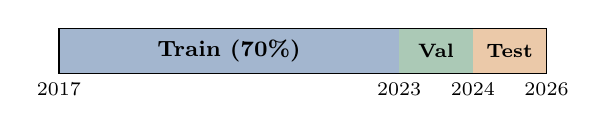
\begin{tikzpicture}[scale=0.72]
\fill[accentblue!40] (0,0) rectangle (6,0.8);
\fill[accentgreen!40] (6,0) rectangle (7.3,0.8);
\fill[accentorange!40] (7.3,0) rectangle (8.6,0.8);
\draw (0,0) rectangle (8.6,0.8);
\node at (3,0.4) {\footnotesize \textbf{Train (70\%)}};
\node at (6.65,0.4) {\scriptsize \textbf{Val}};
\node at (7.95,0.4) {\scriptsize \textbf{Test}};
\node[below] at (0,0) {\scriptsize 2017};
\node[below] at (6,0) {\scriptsize 2023};
\node[below] at (7.3,0) {\scriptsize 2024};
\node[below] at (8.6,0) {\scriptsize 2026};
\end{tikzpicture}

\vspace{0.6cm}
{\scriptsize\raggedright \textbf{Chronological split} --- no shuffling across the temporal boundary.\\ Val and test are genuinely unseen future data.\par}
\end{columns}
\end{frame}

\begin{frame}{Stationary feature engineering}
\begin{columns}[T,onlytextwidth]
\column{0.55\textwidth}
\textbf{Target: log return, not price}
\begin{equation*}
r_t = \ln\!\left(\frac{C_t}{C_{t-1}}\right)
\end{equation*}
\begin{itemize}\small
  \item Approximately stationary
  \item Roughly symmetric around zero
  \item Bounded by daily move distribution
\end{itemize}

\vspace{0.4cm}
\textbf{Reconstruct prices at eval time}
\begin{equation*}
\hat{C}_{t+h} = C_t \cdot \exp\!\left(\sum_{k=1}^{h}\hat{r}_{t+k}\right)
\end{equation*}

\column{0.45\textwidth}
\textbf{All price-level features $\to$ stationary}
\begin{itemize}\small
  \item $\mathrm{Close\_SMA30} = C_t / \mathrm{SMA}_{30,t} - 1$
  \item $\mathrm{Close\_EMA14} = C_t / \mathrm{EMA}_{14,t} - 1$
  \item $\mathrm{MACD\_norm} = \mathrm{MACD}_t / C_t$
  \item $\mathrm{BB\_Width} = 2\sigma_{20,t} / \mu_{20,t}$
  \item RSI-14 (already stationary)
  \item $\mathrm{LogVolume} = \ln(1 + V_t)$
\end{itemize}

\vspace{0.3cm}
\textbf{Halving cycle (sine-cosine)}
\begin{equation*}
\sin\!\left(\tfrac{2\pi d_t}{1460}\right),\ \cos\!\left(\tfrac{2\pi d_t}{1460}\right)
\end{equation*}
\end{columns}
\end{frame}

\begin{frame}{Leak-free normalization}
\begin{columns}[T,onlytextwidth]
\column{0.5\textwidth}
\textbf{The common mistake}
\begin{itemize}\small
  \item Fit scaler on full dataset
  \item Includes test-period extrema
  \item Leaks test statistics into model
\end{itemize}

\vspace{0.4cm}
\textbf{Our fix}
\begin{itemize}\small
  \item \texttt{StandardScaler.fit}($X_{\text{train}}$) only
  \item \texttt{transform}($X_{\text{val}}$, $X_{\text{test}}$)
  \item Target scaler fit on training log returns only
\end{itemize}

\column{0.5\textwidth}
\textbf{Why StandardScaler, not MinMax?}
\begin{equation*}
z = \frac{x - \mu_{\text{train}}}{\sigma_{\text{train}}}
\end{equation*}
\begin{itemize}\small
  \item Robust to extreme values
  \item Better match for heavy-tailed financial data
  \item Doesn't clip unseen future values
\end{itemize}

\vspace{0.3cm}
\begin{block}{Result}
Target distribution stable across train $\to$ val $\to$ test. The model can reach any plausible future value.
\end{block}
\end{columns}
\end{frame}

\begin{frame}{Multi-step sequence construction}
\begin{columns}[T,onlytextwidth]
\column{0.55\textwidth}
\textbf{Sliding-window of $T = 60$ days}
\vspace{0.2cm}
\\ Each sample $\mathbf{X}_i \in \mathbb{R}^{60 \times 17}$
\\ Target $\mathbf{y}_i \in \mathbb{R}^{3}$ = next 3 scaled log returns
\vspace{0.3cm}
\begin{equation*}
(\hat{r}_{t+1}, \hat{r}_{t+2}, \hat{r}_{t+3}) = f(\mathbf{x}_{t-59},\ldots,\mathbf{x}_t)
\end{equation*}

\vspace{0.3cm}
\textbf{Anchor price} = last close in input window
\\[0.1cm] Carried through with each sample for price reconstruction at evaluation.

\column{0.45\textwidth}
\centering
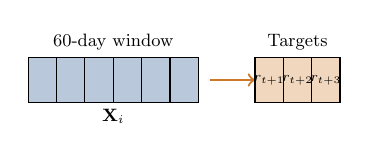
\begin{tikzpicture}[scale=0.72,transform shape]
\foreach \x in {0,...,5} {
  \fill[accentblue!30] (\x*0.5, 0) rectangle (\x*0.5+0.5, 0.8);
  \draw (\x*0.5, 0) rectangle (\x*0.5+0.5, 0.8);
}
\node[above] at (1.5,0.8) {\small 60-day window};
\node[below] at (1.5,0) {\small $\mathbf{X}_i$};
\draw[->, thick, accentorange] (3.2,0.4) -- (4.0,0.4);
\foreach \x in {0,1,2} {
  \fill[accentorange!30] (4+\x*0.5, 0) rectangle (4+\x*0.5+0.5, 0.8);
  \draw (4+\x*0.5, 0) rectangle (4+\x*0.5+0.5, 0.8);
}
\node[above] at (4.75,0.8) {\small Targets};
\node at (4.25,0.4) {\scriptsize $r_{t+1}$};
\node at (4.75,0.4) {\scriptsize $r_{t+2}$};
\node at (5.25,0.4) {\scriptsize $r_{t+3}$};
\end{tikzpicture}

\vspace{0.5cm}
\small Multi-step target discourages memorizing a single noisy horizon and produces smoother trend-aware predictions.
\end{columns}
\end{frame}

% ============================================================
%  PART 3 --- MODEL ARCHITECTURES
% ============================================================

\section{Model Architectures}

\begin{frame}{Four architectures, one pipeline}
\footnotesize
\renewcommand{\arraystretch}{1.3}
\begin{tabular}{L{2.8cm}L{5cm}L{5cm}}
\toprule
\textbf{Model} & \textbf{Key idea} & \textbf{Why we included it} \\
\midrule
DNN + feature gate &
Flatten $60{\times}17$ window; per-feature sigmoid gate re-weights features from sequence mean &
Static baseline; tests whether temporal structure matters \\[0.15cm]

LSTM + temporal attention &
2-layer LSTM; learned attention over all 60 hidden states &
Gold-standard recurrent model for financial sequences \\[0.15cm]

CNN-Transformer &
Two Conv1D blocks $\to$ positional encoding $\to$ 2-layer TransformerEncoder (8 heads) &
Combines local pattern detection with global self-attention \\[0.15cm]

TCN &
4 TemporalBlocks, dilations $2^0,2^1,2^2,2^3$, receptive field $R=31$ &
Paper 2 winner on 1-min data; tests if it transfers to daily \\
\bottomrule
\end{tabular}

\vspace{0.3cm}
\centering
\begin{block}{Unified training protocol}
AdamW ($\mathrm{lr}=10^{-3}$, wd $=10^{-4}$) + Huber loss + cosine annealing + early stopping
\end{block}
\end{frame}

\begin{frame}{Model 1: DNN with feature attention gate}
\begin{columns}[T,onlytextwidth]
\column{0.6\textwidth}
\centering
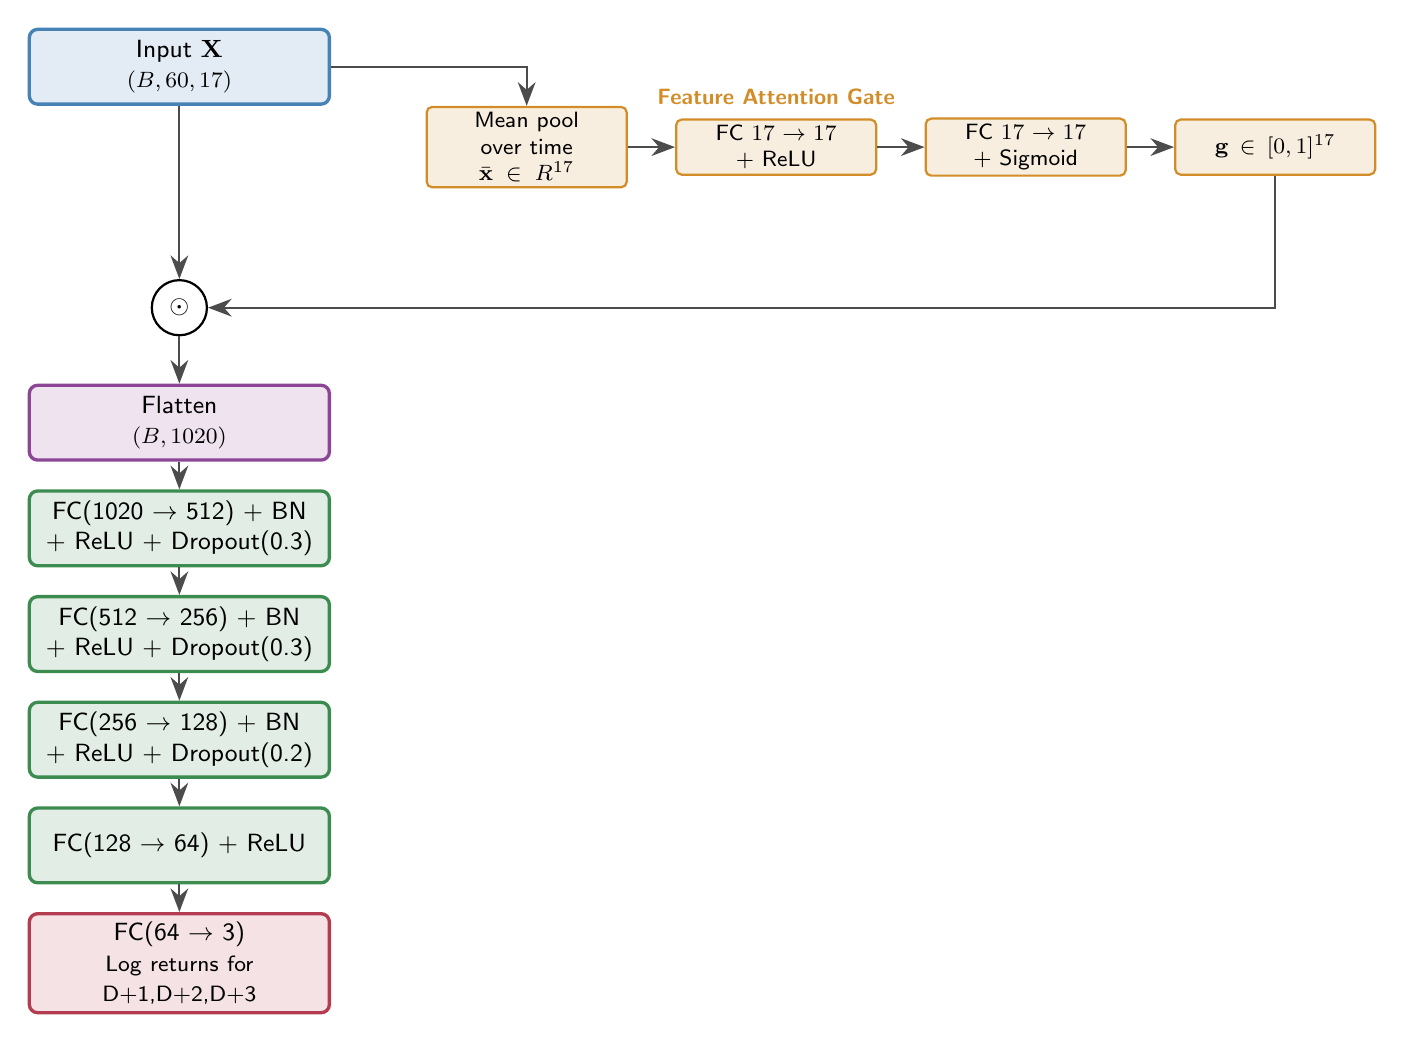
\includegraphics[height=0.78\textheight]{fig_arch_dnn.png}

\column{0.4\textwidth}
\textbf{Feature-attention gate}
\begin{equation*}
\mathbf{g} = \sigma(W_2 \cdot \mathrm{ReLU}(W_1 \cdot \bar{\mathbf{x}}))
\end{equation*}
$\bar{\mathbf{x}}$ = mean activation over 60 time steps
\\[0.1cm] Re-weight input: $\mathbf{x}'_t = \mathbf{g} \odot \mathbf{x}_t$

\vspace{0.4cm}
\textbf{4-layer MLP head}
\begin{itemize}\small
  \item BatchNorm between layers
  \item Dropout 0.2--0.3
  \item Output: 3 log returns
\end{itemize}
\end{columns}
\end{frame}

\begin{frame}{Model 2: LSTM with temporal self-attention}
\begin{columns}[T,onlytextwidth]
\column{0.6\textwidth}
\centering
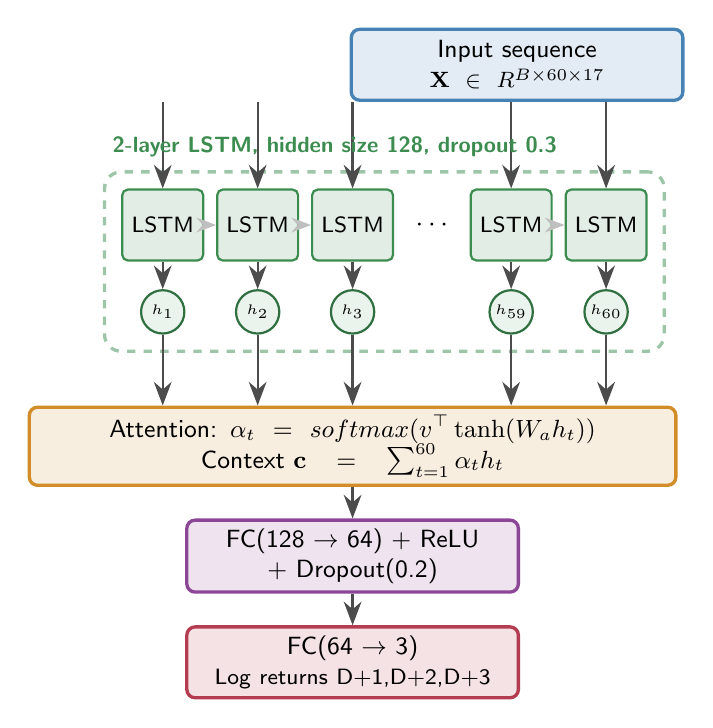
\includegraphics[height=0.78\textheight]{fig_arch_lstm.png}

\column{0.4\textwidth}
\textbf{LSTM cell update}
\begin{align*}
f_t &= \sigma(W_f[h_{t-1}, x_t] + b_f) \\
i_t &= \sigma(W_i[h_{t-1}, x_t] + b_i) \\
\tilde{c}_t &= \tanh(W_c[h_{t-1}, x_t] + b_c) \\
c_t &= f_t \odot c_{t-1} + i_t \odot \tilde{c}_t \\
h_t &= o_t \odot \tanh(c_t)
\end{align*}

\vspace{0.2cm}
\textbf{Attention pooling}
\begin{equation*}
\mathbf{c} = \sum_{t=1}^{60} \alpha_t h_t
\end{equation*}
\end{columns}
\end{frame}

\begin{frame}{Model 3: CNN-Transformer hybrid}
\begin{columns}[T,onlytextwidth]
\column{0.55\textwidth}
\centering
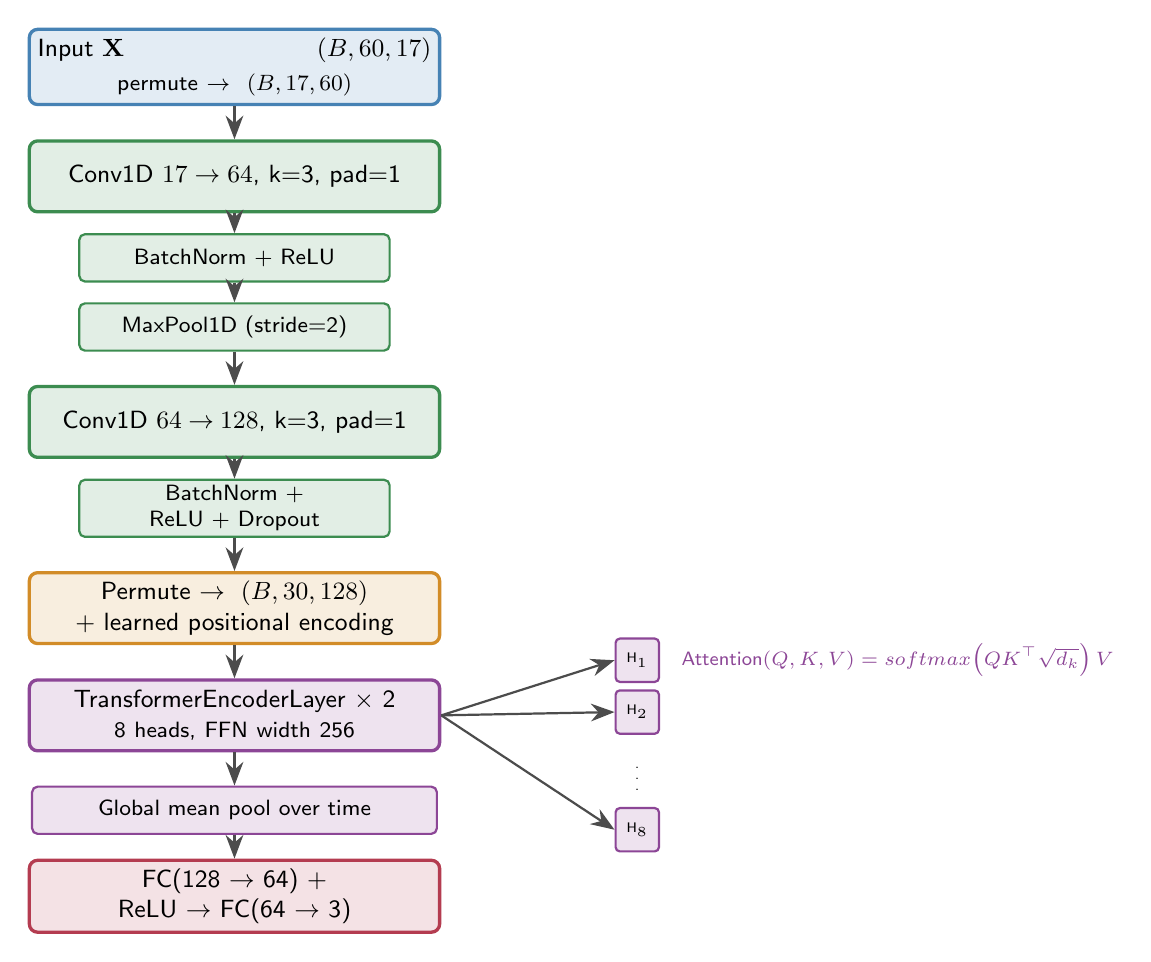
\includegraphics[height=0.78\textheight]{fig_arch_cnntr.png}

\column{0.45\textwidth}
\textbf{Stage 1: CNN local features}
\begin{itemize}\small
  \item Conv1D $17 \to 64$, MaxPool(2)
  \item Conv1D $64 \to 128$
  \item Compresses $60 \to 30$ time steps
\end{itemize}

\vspace{0.3cm}
\textbf{Stage 2: Transformer global}
\begin{itemize}\small
  \item Learned positional encoding
  \item 2 layers, 8 attention heads
  \item Feed-forward width 256
\end{itemize}
\begin{equation*}
\mathrm{Attn}(Q,K,V) = \mathrm{softmax}\!\left(\tfrac{QK^\top}{\sqrt{d_k}}\right)V
\end{equation*}
\end{columns}
\end{frame}

\begin{frame}{Model 4: Temporal Convolutional Network}
\begin{columns}[T,onlytextwidth]
\column{0.65\textwidth}
\centering
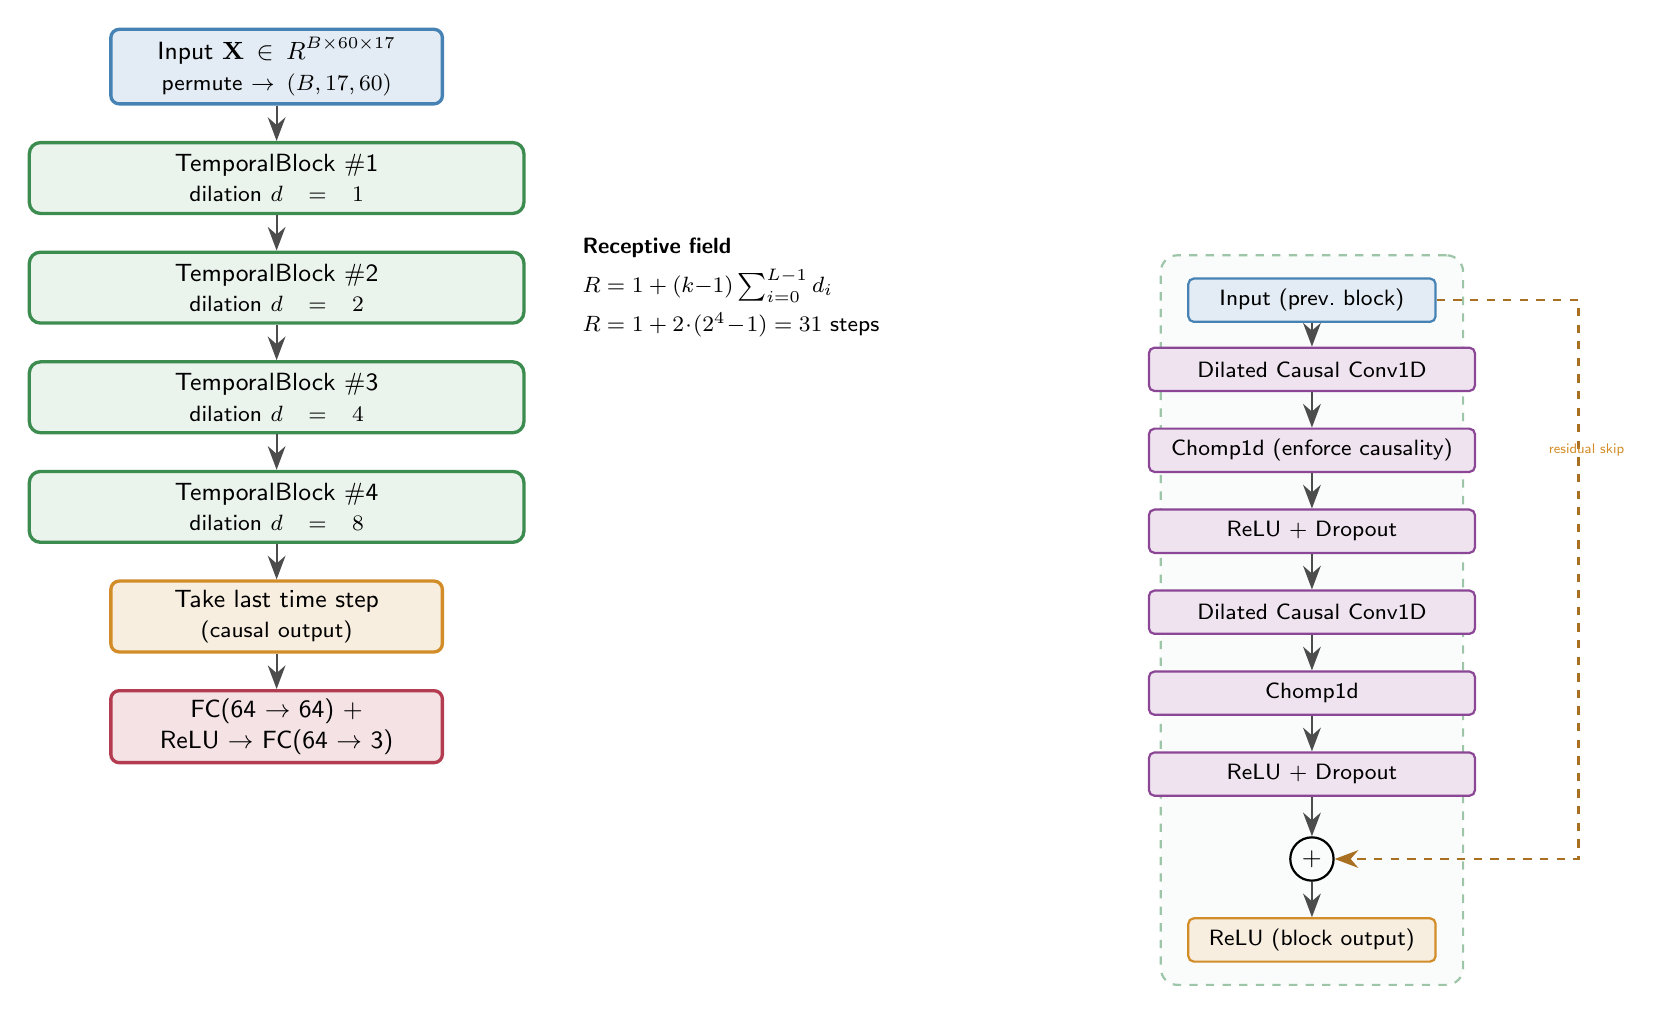
\includegraphics[width=\linewidth]{fig_arch_tcn.png}

\column{0.35\textwidth}
\textbf{Dilated causal conv}
\begin{equation*}
y[t] = \sum_{i=0}^{k-1} w[i] \cdot x[t - d \cdot i]
\end{equation*}

\vspace{0.2cm}
\textbf{Receptive field}
\begin{equation*}
R = 1 + (k-1)(2^L - 1) = 31
\end{equation*}

\vspace{0.2cm}
\begin{itemize}\small
  \item Fully parallelizable
  \item No vanishing gradients
  \item Strict causality preserved
\end{itemize}
\end{columns}
\end{frame}

\begin{frame}{Training protocol}
\begin{columns}[T,onlytextwidth]
\column{0.55\textwidth}
\textbf{Huber loss (robust to shock days)}
\begin{equation*}
\mathcal{L}_\mathrm{H}(y,\hat{y}) =
\begin{cases}
\frac{1}{2}(y-\hat{y})^2 & |y-\hat{y}| \le \delta \\
\delta(|y-\hat{y}| - \tfrac{1}{2}\delta) & \text{otherwise}
\end{cases}
\end{equation*}

\begin{itemize}\small
  \item Quadratic for small residuals
  \item Linear for large residuals
  \item Doesn't blow up on shock days
\end{itemize}

\column{0.45\textwidth}
\textbf{Optimizer \& scheduling}
\begin{itemize}\small
  \item AdamW, lr $10^{-3}$, wd $10^{-4}$
  \item Cosine annealing over 100 epochs
  \item Early stopping, patience 15
  \item Gradient clipping at norm 1.0
  \item Batch size 64
  \item Sample-level shuffle on train loader
\end{itemize}

\vspace{0.3cm}
\begin{block}{All four models, identical protocol}
Architecture differences are the only variable.
\end{block}
\end{columns}
\end{frame}

\begin{frame}{Ensemble pipeline}
\centering
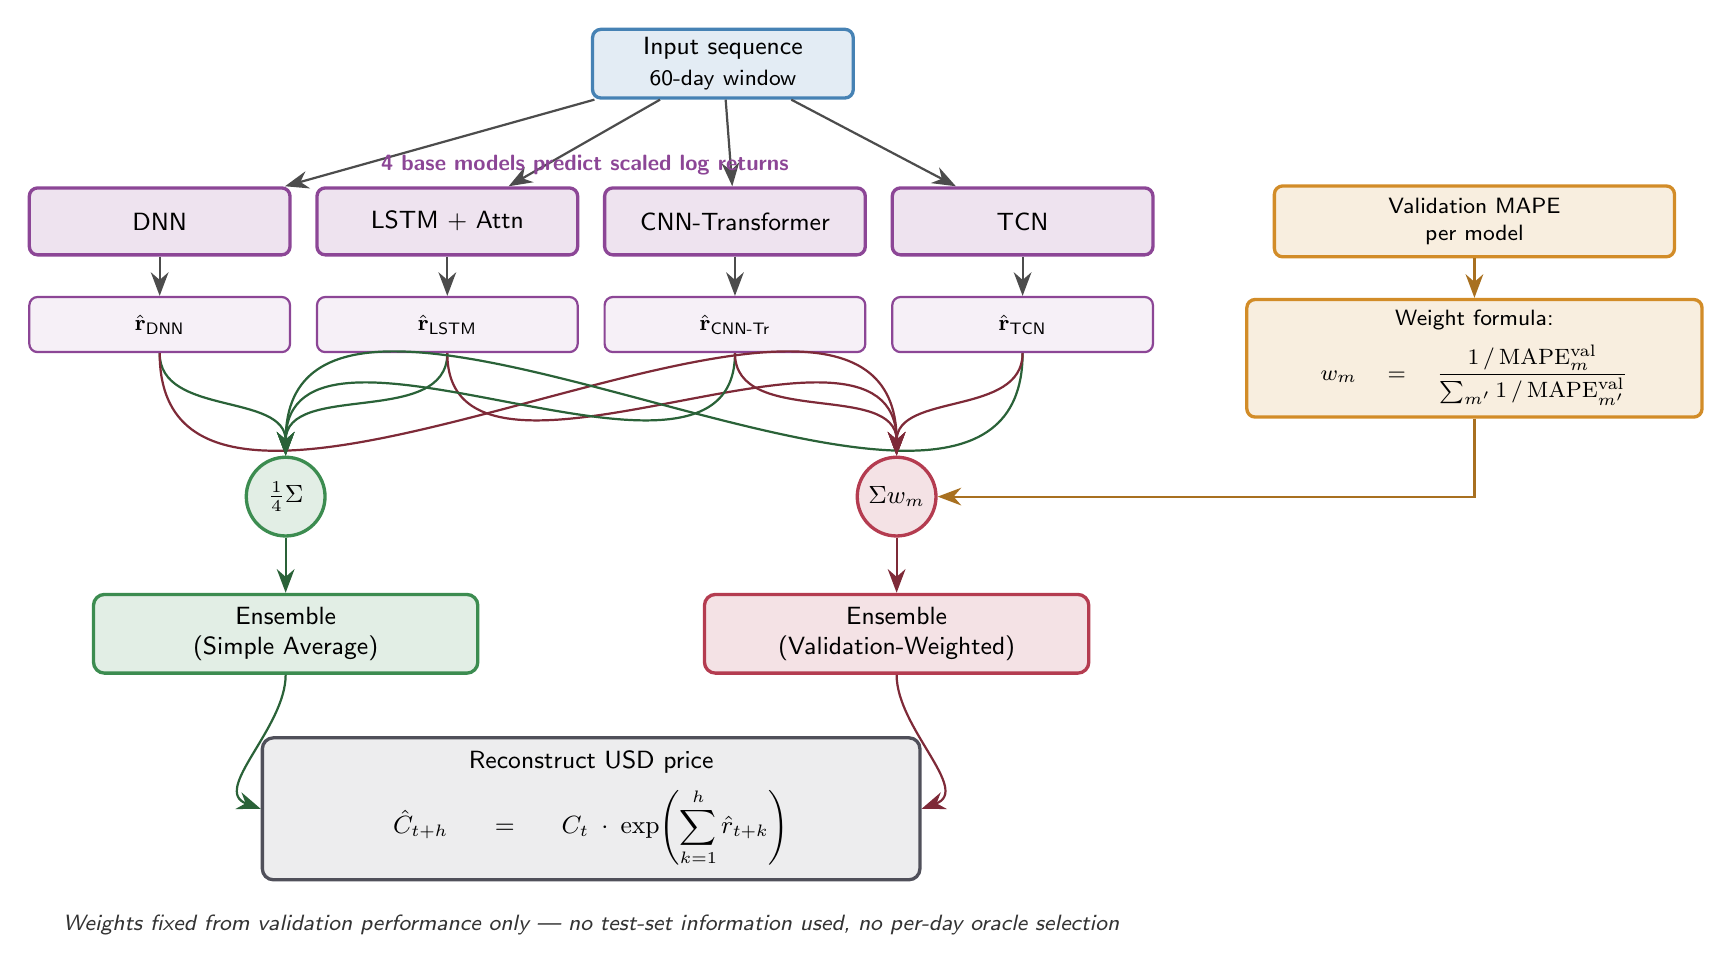
\includegraphics[width=0.86\textwidth]{fig_ensemble.png}
\end{frame}

\begin{frame}{Two ensembles, no oracle}
\textbf{Simple Average:} mean of 4 model outputs at each horizon.
\vspace{0.3cm}
\\ \textbf{Weighted by Validation MAPE:}
\begin{equation*}
w_m = \frac{1/\mathrm{MAPE}_m^{\mathrm{val}}}{\sum_{m'} 1/\mathrm{MAPE}_{m'}^{\mathrm{val}}}
\end{equation*}

\vspace{0.4cm}
\begin{block}{Critical distinction from CFA (Wu et al.\ 2025)}
Weights come from \textbf{validation} only, never test.\\
No per-day selection across combinations.
\end{block}

\vspace{0.3cm}
\centering
\small Both ensemble outputs go through the same price-reconstruction step\\ as individual models: $\hat{C}_{t+h} = C_t \cdot \exp(\sum_k \hat{r}_{t+k})$.
\end{frame}

% ============================================================
%  PART 4 --- EVALUATION & RESULTS
% ============================================================

\section{Evaluation \& Results}

\begin{frame}{Evaluation metric suite}
\begin{columns}[T,onlytextwidth]
\column{0.5\textwidth}
\textbf{Error magnitude}
\begin{equation*}
\mathrm{RMSE} = \sqrt{\tfrac{1}{N}\sum (y_i - \hat{y}_i)^2}
\end{equation*}
\begin{equation*}
\mathrm{MAE} = \tfrac{1}{N}\sum |y_i - \hat{y}_i|
\end{equation*}
\begin{equation*}
\mathrm{MAPE} = \tfrac{100}{N}\sum \left|\tfrac{y_i - \hat{y}_i}{y_i}\right|
\end{equation*}

\column{0.5\textwidth}
\textbf{Variance explained}
\begin{equation*}
R^2 = 1 - \tfrac{\sum (y_i - \hat{y}_i)^2}{\sum (y_i - \bar{y})^2}
\end{equation*}

\vspace{0.3cm}
\textbf{Directional accuracy}
\begin{equation*}
\mathrm{DA} = \tfrac{1}{N}\sum \mathbb{1}[(\hat{y}_i - a_i)(y_i - a_i) > 0]
\end{equation*}
where $a_i$ = anchor price.
\\[0.2cm] Plus: \textbf{Precision, Recall, F1} for up-moves.
\end{columns}

\vspace{0.3cm}
\begin{block}{Why directional accuracy matters}
RMSE/MAPE tell you \emph{how far off} you are. DA tells you \emph{whether you called the direction right} --- which is what a trader actually cares about.
\end{block}
\end{frame}

\begin{frame}{The crucial naive baseline}
\begin{block}{Naive random-walk: $\hat{y}_{t+1} = y_t$}
\centering
\footnotesize
\begin{tabular}{lcccc}
\toprule
\textbf{Horizon} & \textbf{RMSE} & \textbf{MAE} & \textbf{MAPE} & $R^2$ \\
\midrule
Day+1 & \$2{,}152 & \$1{,}557 & 1.68\% & 0.981 \\
Day+2 & \$2{,}950 & \$2{,}223 & 2.40\% & 0.964 \\
Day+3 & \$3{,}534 & \$2{,}714 & 2.93\% & 0.948 \\
\bottomrule
\end{tabular}
\end{block}

\vspace{0.3cm}
\begin{alertblock}{Critical insight}
On a \textbf{trending test period}, ``today = tomorrow'' is already an extremely strong heuristic.
\\[0.1cm] Any honest deep learning paper on daily BTC must clear \textbf{this} bar, not just beat a random classifier.
\end{alertblock}
\end{frame}

\begin{frame}{Static-split results --- Day+1}
\footnotesize
\begin{center}
\begin{tabular}{lccccc}
\toprule
\textbf{Model} & \textbf{RMSE (\$)} & \textbf{MAE (\$)} & \textbf{MAPE (\%)} & $R^2$ & \textbf{DirAcc} \\
\midrule
Naive baseline        & 2{,}152 & 1{,}557 & 1.68 & 0.981 & 0.491 \\
DNN                   & 2{,}168 & 1{,}583 & 1.71 & 0.980 & 0.501 \\
LSTM                  & 2{,}154 & 1{,}565 & 1.69 & 0.981 & 0.503 \\
CNN-Transformer       & 2{,}182 & 1{,}605 & 1.73 & 0.980 & 0.513 \\
\rowcolor{accentgreen!20}
\textbf{TCN}          & \textbf{2{,}144} & 1{,}571 & 1.69 & \textbf{0.981} & 0.505 \\
Ensemble (Avg)        & 2{,}146 & \textbf{1{,}561} & \textbf{1.69} & 0.981 & 0.507 \\
Ensemble (Wtd)        & 2{,}146 & 1{,}561 & 1.69 & 0.981 & 0.505 \\
\bottomrule
\end{tabular}
\end{center}

\vspace{0.3cm}
\begin{alertblock}{The honest read}
\begin{itemize}\small
  \item All models are within \$40 RMSE of the naive baseline.
  \item The previous version of this project got $R^2 = -16$. The fact that every model now tracks the baseline is a \textbf{major recovery}.
  \item Static split alone is not a defensible headline --- we need walk-forward.
\end{itemize}
\end{alertblock}
\end{frame}

\begin{frame}{Walk-forward validation: the headline result}
\begin{columns}[T,onlytextwidth]
\column{0.42\textwidth}
\textbf{Protocol}
\begin{itemize}\small
  \item Initial train: 24 months
  \item Step size: 4 months
  \item Evaluation: 1 month / step
  \item 20 folds, April 2019 -- August 2025
  \item Each fold retrains on expanding window
\end{itemize}

\vspace{0.3cm}
\begin{block}{\color{white}Headline}
\large\centering
\textbf{Avg MAPE: 2.23\%}
\\ LSTM and TCN identical.
\end{block}

\column{0.58\textwidth}
\centering
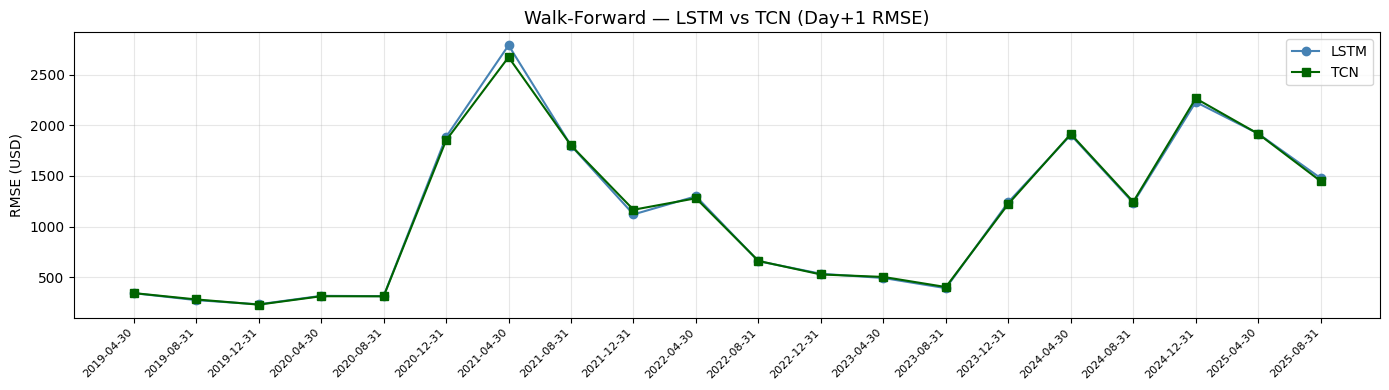
\includegraphics[width=\linewidth]{fig07_walkforward_comparison.png}
\\[0.1cm] \scriptsize LSTM vs TCN walk-forward RMSE across 20 folds.
\end{columns}
\end{frame}

\begin{frame}{Walk-forward --- regime dependence}
\centering
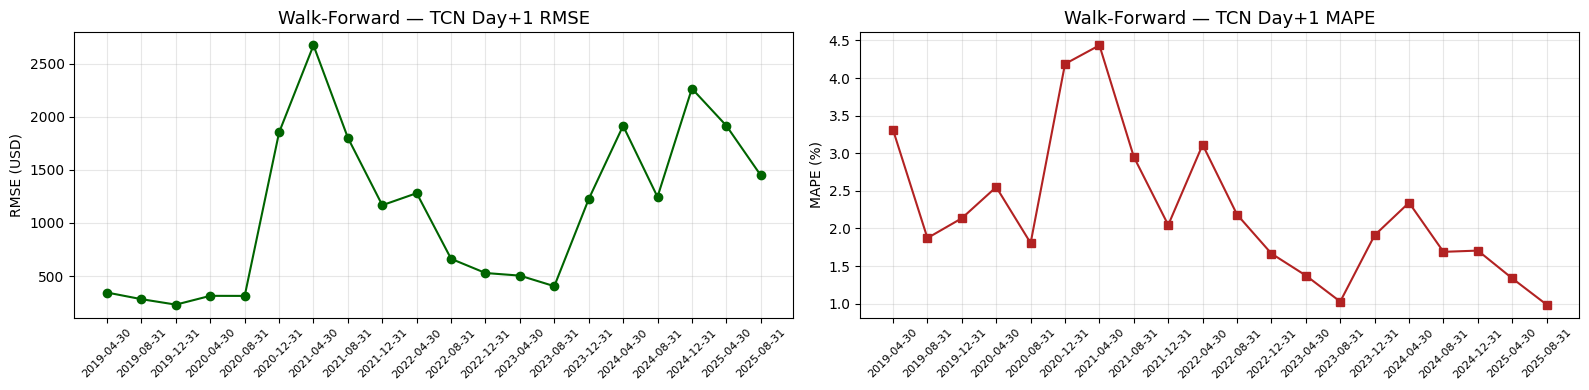
\includegraphics[width=0.9\textwidth,height=0.31\textheight,keepaspectratio]{fig06_walkforward_tcn.png}

\vspace{0.15cm}
{\large\textbf{Per-fold MAPE ranges from 0.99\% to 4.64\%}}
\begin{itemize}\small
  \item 2019-08: 1.79\% (calm)
  \item \textcolor{accentred}{\textbf{2021-04: 4.64\% (bull-run peak)}}
  \item 2022-08: 2.16\% (recovering)
  \item 2023-08: 0.99\% (low-vol)
  \item 2024-12: 1.66\% (ETF-era)
  \item 2025-08: 0.99\% (stable)
\end{itemize}

\vspace{0.15cm}
\begin{block}{Regime sensitivity}
\scriptsize Volatile regimes (bull peaks, sharp drawdowns) dominate the error budget --- future work: regime-conditional models.
\end{block}
\end{frame}

\begin{frame}{Are the differences statistically significant?}
\footnotesize
\begin{center}
\textbf{Diebold--Mariano test on Day+1 squared-error loss}
\\[0.2cm]
\begin{tabular}{lcccc}
\toprule
\textbf{A} vs \textbf{B} & \textbf{DM stat} & \textbf{p-value} & \textbf{Significant?} \\
\midrule
Ensemble-Avg vs DNN                & $-2.05$ & 0.041 & \textcolor{accentgreen}{\textbf{Yes *}} \\
Ensemble-Avg vs CNN-Transformer    & $-2.60$ & 0.009 & \textcolor{accentgreen}{\textbf{Yes **}} \\
Ensemble-Wtd vs DNN                & $-2.05$ & 0.041 & \textcolor{accentgreen}{\textbf{Yes *}} \\
Ensemble-Wtd vs CNN-Transformer    & $-2.60$ & 0.009 & \textcolor{accentgreen}{\textbf{Yes **}} \\
CNN-Transformer vs LSTM            & $+1.67$ & 0.096 & Marginal \\
TCN vs CNN-Transformer             & $-1.49$ & 0.136 & No \\
TCN vs LSTM                        & $-0.60$ & 0.551 & No \\
LSTM vs DNN                        & $-0.79$ & 0.428 & No \\
\bottomrule
\end{tabular}
\end{center}

\vspace{0.3cm}
\begin{block}{What this tells us}
\begin{itemize}\small
  \item Ensembles are significantly better than DNN and CNN-Transformer.
  \item TCN, LSTM and ensembles are \textbf{statistically tied}.
  \item Architecture choice, beyond a reasonable baseline, is \textbf{second-order} to pipeline hygiene.
\end{itemize}
\end{block}
\end{frame}

\begin{frame}{Feature-group ablation}
\begin{columns}[T,onlytextwidth]
\column{0.55\textwidth}
\centering
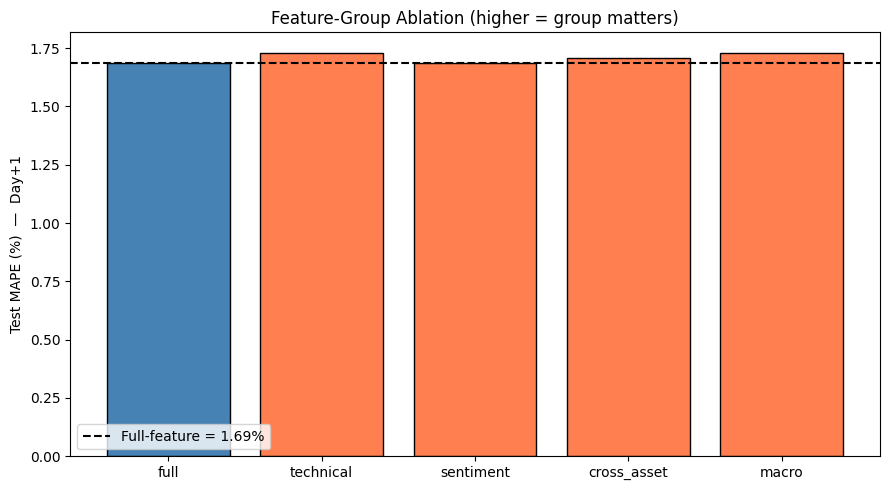
\includegraphics[width=\linewidth]{fig08_ablation.png}

\column{0.45\textwidth}
\textbf{Drop one group, retrain TCN}
\\[0.1cm] \small
\begin{tabular}{lr}
\toprule
\textbf{Dropped} & \textbf{$\Delta$ MAPE} \\
\midrule
Technical (9 feats)  & +0.045 \\
Macro (2 feats)      & +0.043 \\
Cross-asset (5 feats)& +0.019 \\
Sentiment (1 feat)   & $-$0.001 \\
\bottomrule
\end{tabular}

\vspace{0.3cm}
\begin{alertblock}{Finding}
\footnotesize
The Fear \& Greed Index --- popular in the literature --- contributes \textbf{essentially nothing} once other features are present.
\end{alertblock}
\end{columns}
\end{frame}

\begin{frame}{Where we land in the literature}
\footnotesize
\begin{center}
\begin{tabular}{lllc}
\toprule
\textbf{Study} & \textbf{Method} & \textbf{MAPE} & \textbf{Leak-free?} \\
\midrule
Hamayel \& Owda (2021) & GRU & 0.245\% & Yes \\
Jin \& Li (2023)       & VMD-AGRU-RESVMD-LSTM & 0.394\% & Yes \\
Kim et al.\ (2022)     & SAM-LSTM + on-chain  & 1.33\% & Yes \\
Zhang et al.\ (2022)   & SDAE-B               & 1.60\% & Yes \\
\rowcolor{accentgreen!20}
\textbf{This work}     & \textbf{LSTM / TCN walk-forward} & \textbf{2.23\%} & \textbf{Yes} \\
Chen (2023)            & Random Forest        & 3.29\% & Yes \\
Ji et al.\ (2019)      & DNN                  & 3.61\% & Yes \\
Ye et al.\ (2022)      & LSTM+GRU + Twitter   & 4.49\% & Yes \\
\midrule
\rowcolor{accentred!15}
Wu et al.\ (2025)      & CFA (104 combinations)   & 0.19\% & \textcolor{accentred}{Oracle selection} \\
\rowcolor{accentred!15}
Jin et al.\ (2025)     & TCN on 1-minute data     & 0.002\% & \textcolor{accentred}{Different horizon} \\
\bottomrule
\end{tabular}
\end{center}

\vspace{0.2cm}
\begin{block}{Positioning}
Our 2.23\% lands squarely in the honest, leak-free band between 1.3\% and 3.6\% --- comparable to Zhang (1.60\%) and Chen (3.29\%).
\end{block}
\end{frame}

\begin{frame}{Real-time inference}
\begin{columns}[T,onlytextwidth]
\column{0.5\textwidth}
\textbf{Live predictions, April 2026}
\\[0.2cm] Anchor (latest close): \textbf{\$77{,}971.20}
\\[0.15cm]
\small
\begin{tabular}{ll}
\toprule
\textbf{Model} & \textbf{Day+1 forecast} \\
\midrule
DNN              & \$78{,}055.43 \\
LSTM             & \$77{,}949.70 \\
CNN-Transformer  & \$77{,}962.61 \\
TCN              & \$77{,}964.08 \\
\rowcolor{accentgreen!15}
Ensemble (Avg)   & \$77{,}982.95 \\
Ensemble (Wtd)   & \$77{,}982.77 \\
\bottomrule
\end{tabular}

\vspace{0.2cm}
\scriptsize CNN-Transformer 95\% CI: \$77{,}929 -- \$77{,}988

\column{0.5\textwidth}
\textbf{MC Dropout for uncertainty}
\begin{itemize}\small
  \item 100 stochastic forward passes
  \item Dropout kept on at inference
  \item $\pm 1.96\sigma$ gives 95\% prediction interval
\end{itemize}

\vspace{0.3cm}
\begin{block}{Takeaway}
\footnotesize
All six predictions cluster within 0.1\% of anchor. Narrow spread is consistent with DM findings: architectures converge under calm regimes.
\end{block}
\end{columns}
\end{frame}

\begin{frame}{Directional accuracy reality check}
\begin{center}
\footnotesize
\begin{tabular}{lccc}
\toprule
\textbf{Model} & \textbf{Day+1 DA} & \textbf{Day+2 DA} & \textbf{Day+3 DA} \\
\midrule
DNN & 50.1\% & 51.3\% & 52.1\% \\
LSTM & 50.3\% & 49.7\% & 53.1\% \\
CNN-Transformer & 51.3\% & 50.3\% & 51.1\% \\
TCN & 50.5\% & 53.1\% & 53.5\% \\
Ensemble (Avg) & 50.7\% & 52.5\% & 55.1\% \\
\bottomrule
\end{tabular}
\end{center}

\vspace{0.3cm}
\begin{block}{What this means}
\begin{itemize}\small
  \item Daily BTC direction is very close to unpredictable (fair coin = 50\%).
  \item McNally et al.\ (2018): 52.78\% with LSTM on daily BTC.
  \item Jin et al.\ (2025): 53.01\% single-factor TCN on minute data.
  \item Anyone claiming $>$60\% daily directional accuracy without threshold filtering is doing something suspicious.
\end{itemize}
\end{block}
\end{frame}

% ============================================================
%  CONCLUSION
% ============================================================

\section{Conclusion}

\begin{frame}{Contributions \& findings}
\begin{enumerate}
  \item \textbf{Stationary-target design} fixed negative $R^2$ failure. The single most important change in the project.
  \item \textbf{Walk-forward MAPE 2.23\%} over 20 folds and six years of diverse market regimes --- the defensible headline.
  \item \textbf{No single model is significantly best} (DM $p > 0.05$); architectural choice is second-order to pipeline quality.
  \item \textbf{Sentiment features contribute nothing} (ablation); macro + technical features dominate.
  \item \textbf{Directional accuracy $\approx 50\%$} --- daily BTC direction is essentially unpredictable with these features.
  \item \textbf{Ensembles are significantly better} than the weakest individual models but not the best.
\end{enumerate}
\end{frame}

\begin{frame}{Limitations \& future work}
\begin{columns}[T,onlytextwidth]
\column{0.5\textwidth}
\textbf{Limitations}
\begin{itemize}\small
  \item Per-fold MAPE varies 0.99\%--4.64\% (regime-dependent)
  \item Transaction costs not modelled
  \item MC Dropout under-covers (79\% vs nominal 95\%)
  \item Sentiment pipeline under-exploited
\end{itemize}

\column{0.5\textwidth}
\textbf{Future work}
\begin{itemize}\small
  \item Regime-conditional models (volatility-aware)
  \item Higher-frequency extension (hourly / minute)
  \item FinBERT real-time news scoring
  \item Quantile regression or conformal prediction for calibrated CIs
  \item Trading-strategy backtesting with costs
\end{itemize}
\end{columns}

\vspace{0.5cm}
\centering
\begin{block}{Take-home}
\centering
\textbf{Pipeline hygiene $>$ architectural novelty.}
\\[0.1cm] Stationary targets, train-only scaling, and walk-forward evaluation matter more than which neural network you pick.
\end{block}
\end{frame}

% =========== THANK YOU ======================================
\begin{frame}
\begin{center}
\vspace{1cm}
{\LARGE\bfseries\color{accentblue} Thank You!}

\vspace{1.2cm}
{\Large Questions?}

\vspace{1.5cm}
\normalsize
Shamsa Alsuwaidi \quad $\cdot$ \quad
Saeeda Amer \quad $\cdot$ \quad
Amna Aljaroodi

\vspace{0.5cm}
\small MAI 604 --- Deep Learning \quad $\cdot$ \quad April 2026
\end{center}
\end{frame}

% =========== BACKUP =========================================
\appendix
\section{Backup Slides}

\begin{frame}{Backup: full static-split metrics (all horizons)}
\footnotesize
\centering
\begin{tabular}{llccccc}
\toprule
\textbf{Model} & \textbf{Horizon} & \textbf{RMSE} & \textbf{MAE} & \textbf{MAPE} & $R^2$ & \textbf{DA} \\
\midrule
\multirow{3}{*}{DNN} & D+1 & 2168 & 1583 & 1.71 & 0.980 & 0.501 \\
 & D+2 & 3002 & 2269 & 2.45 & 0.962 & 0.513 \\
 & D+3 & 3612 & 2744 & 2.96 & 0.946 & 0.521 \\
\midrule
\multirow{3}{*}{LSTM} & D+1 & 2154 & 1565 & 1.69 & 0.981 & 0.503 \\
 & D+2 & 2955 & 2241 & 2.42 & 0.964 & 0.497 \\
 & D+3 & 3542 & 2718 & 2.93 & 0.948 & 0.531 \\
\midrule
\multirow{3}{*}{TCN} & D+1 & 2144 & 1571 & 1.69 & 0.981 & 0.505 \\
 & D+2 & 2950 & 2236 & 2.41 & 0.964 & 0.531 \\
 & D+3 & 3543 & 2725 & 2.93 & 0.948 & 0.535 \\
\bottomrule
\end{tabular}
\end{frame}

\begin{frame}{Backup: training curves}
\centering
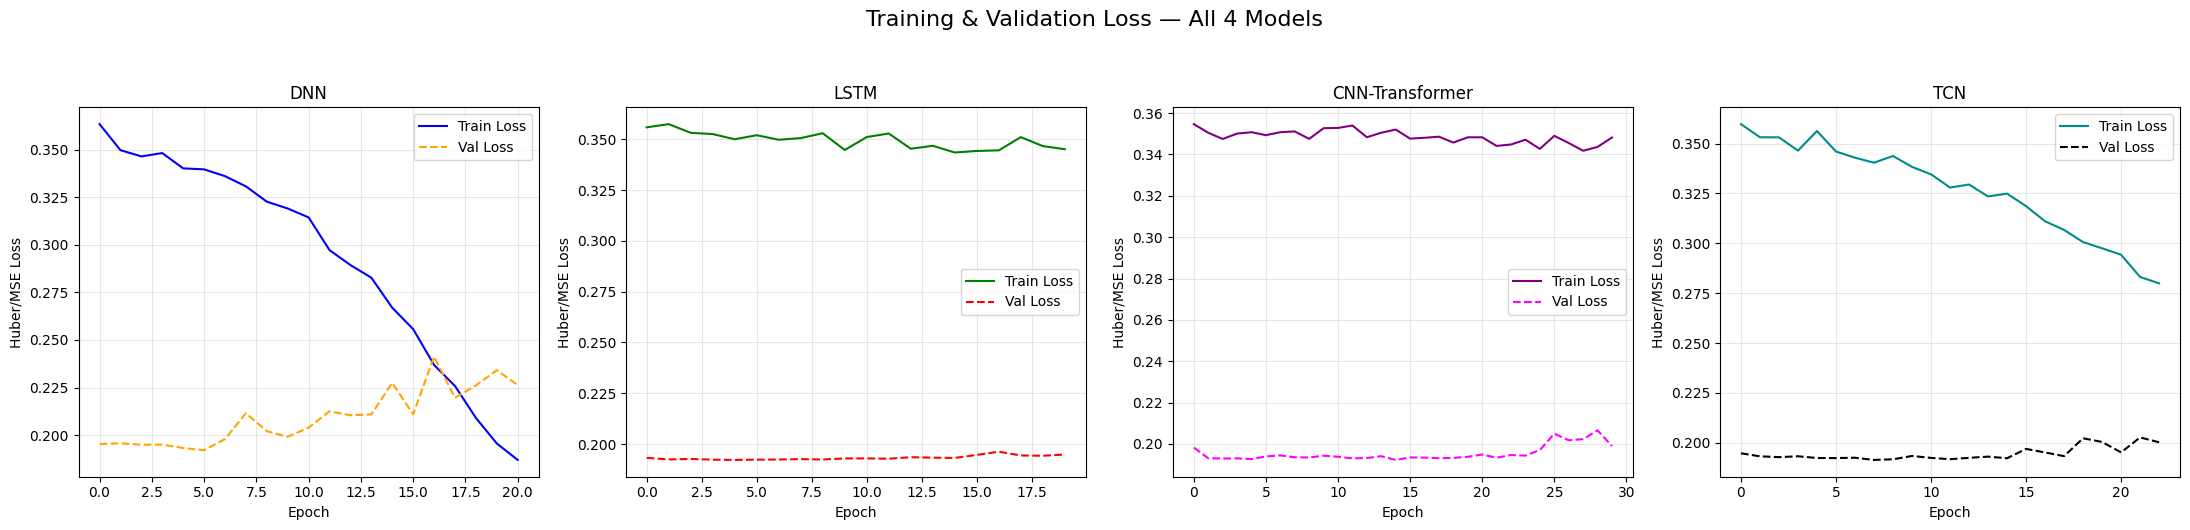
\includegraphics[width=0.85\textwidth]{fig02_loss_curves.png}
\end{frame}

\begin{frame}{Backup: predictions vs actual}
\centering
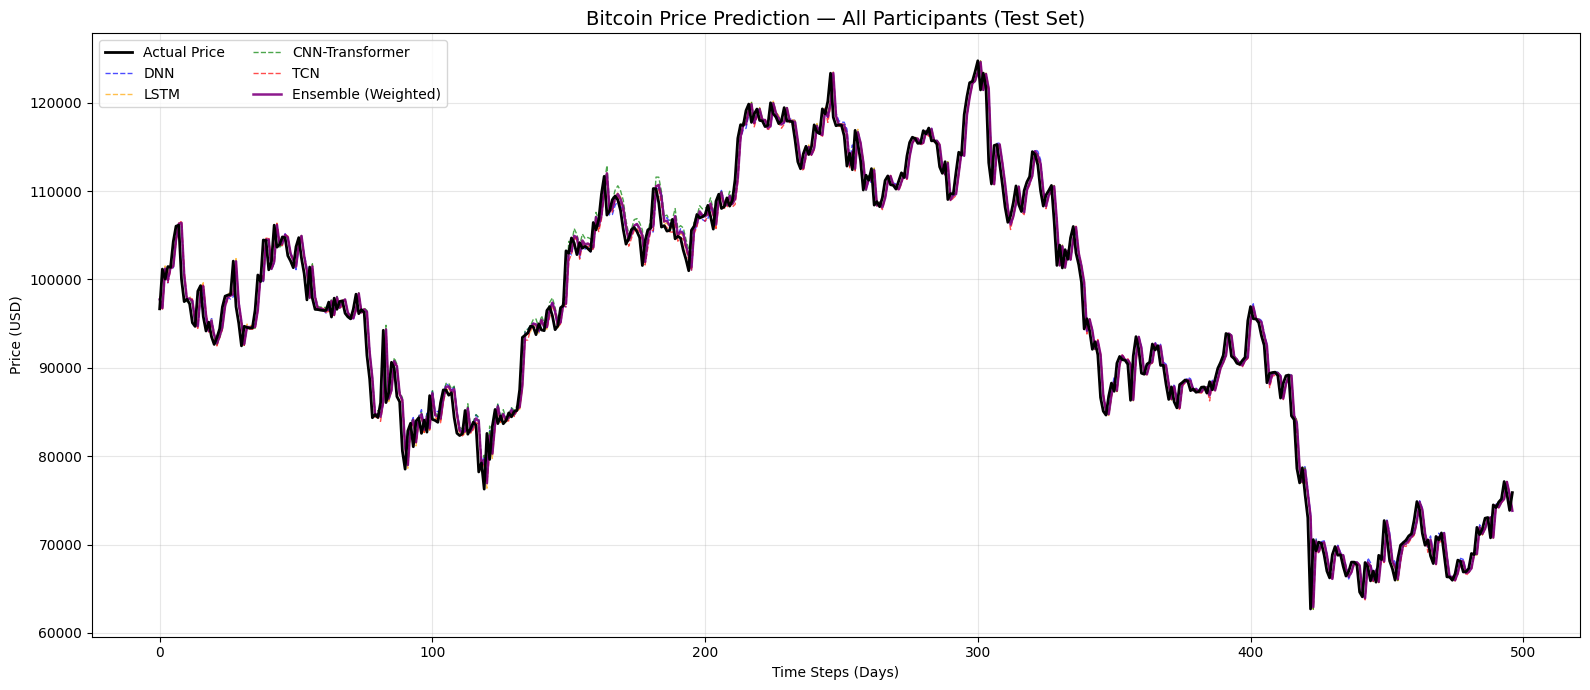
\includegraphics[width=0.95\textwidth]{fig03_predictions_vs_actual.png}
\end{frame}

\begin{frame}{Backup: per-fold walk-forward (LSTM)}
\centering
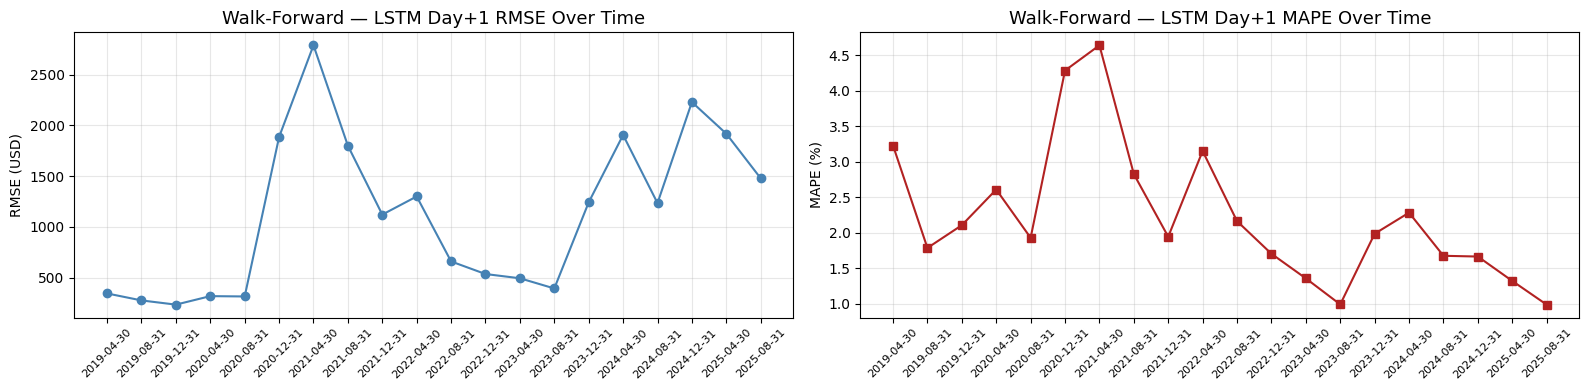
\includegraphics[width=0.95\textwidth]{fig05_walkforward_lstm.png}
\end{frame}

\end{document}
